\documentclass{article}

\usepackage{amsmath}
\usepackage{amssymb}
\usepackage{graphicx}

\DeclareMathOperator*{\argmax}{arg\,max}

\begin{document}

\title{Assignment 1}
\author{Cameron Salisbury}

\maketitle

\section{Introduction}

In this report I will describe my implementation of the Spherical K-Means algorithm to extract features from images based on the description in the paper~\cite{paper}. This implementation has been written Java using the WEKA API~\cite{weka}. This report will also contain some result generated from the algorithm along with a discussion on these results.

\section{Method}

This algorithm is implemented as a filter in WEKA~\cite{weka} and all matrix and vector maths is done using the MTJ library~\cite{matrix_lib}.

\subsection{Initialization}

The spherical K-Means algorithm is described in the paper~\cite{paper} in section 2 and is  split into two subsections. The part of the algorithm described in the first subsection, "Pre-processing", was already implemented, so I just implemented the part of the algorithm described in the "Initialization" subsection. That part of the algorithm that was already implemented extracted a user specified number of random square patches of size $p\textrm{-by-}p$, where $p$ is a user specified size value. The red, green and blue values of the of the pixels in the extracted patches were then used to form vectors $x^{(i)} \in \mathbb{R}^n$, where $n$ is the number of values extracted from the patch, which were normalised as per the equation described in the paper with $\epsilon_{\mathrm{norm}}=10$:
\[
x^{(i)} := \frac{x^{(i)} - \mathrm{mean} \left( x^{(i)} \right) }{\sqrt{\mathrm{var} \left( x^{(i)} + 10 \right) }}, \forall i
\]
These vectors where then used to construct the matrix $X \in \mathbb{R}^{n \times m}$, where $m$ is the number of patches, and that data is then whitened as per the equation described in the paper with $\epsilon_{\mathrm{zca}}=0.1$:
\[
[V,D] := \mathrm{eig} \left( \mathrm{cov} \left( X \right) \right) ; \textrm{ // So } VDV^{\mathrm{T}} = \mathrm{cov} \left( X \right)
\]\[
X := V \left( D + 0.1 \boldsymbol{I} \right) ^{-1/2} V^{\mathrm{T}} X
\]
By using these two processes to pre-process the data we will get better results from the K-means algorithm.

\paragraph*{}

The next part of the algorithm, which I implemented, generates the centroids which will be used to extract features from the images. To begin with a matrix $\mathcal{D} \in \mathbb{R}^{n \times k}$, where $k$ is the number of centroids specified by the user, is filled with random values sampled from a normal distribution and then each column in the $\mathcal{D}$ is normalised. This matrix $\mathcal{D}$ is our dictionary of centroids, where each column is one of our centroids on the unit sphere. We now need to optimise this dictionary. This starts by calculating the matrix $S \in \mathbb{R}^{k \times m}$:
\[
S := \mathcal{D}^{\mathrm{T}} X
\]
giving us a matrix where each column represents one of the patches in $X$ and each value in that column is the dot product between the patch and centroid. As a dot product is minimised when two vectors are orthogonal and maximised when they are collinear, we can think of these values are representing how closely the patch matches the centroid. So we then modify $S$ to keep only the largest value absolute in each column:
\[
s^{(i)}_{j} := 
\begin{cases}
s^{(i)}_j & \textrm{if } j = \argmax\limits_{l} \left| s^{(i)}_l \right| \\
0 & \textrm{otherwise}
\end{cases}
, \forall i,j
\]
giving us a matrix that assigns each patch to the centroid it matches most closely.

\paragraph{}

In the paper it suggests iterating a fixed number of time, saying 10 should be enough, but my algorithm takes a different approach and calculates the sum of squared error:
\[
\mathrm{SSE} = \left\lVert \mathcal{D}S - X \right\rVert_{\mathrm{F}}^{2}
\]
and checks if the sum of squared errors this iteration, $\mathrm{SSE_{new}}$, has changed enough since the last iteration, $\mathrm{SSE_{old}}$, by checking if:
\[
\frac{\mathrm{SSE_{old}} - \mathrm{SSE_{new}}}{\mathrm{SSE_{old}}} < 10^{-12}
\]
Because the algorithm converges this condition should eventually be meet, stopping the iteration process, but there is also a hard limit of 200 iterations (although this limit has never been reached on any test data).

\paragraph{}

The next step is to replace empty centroids as recommended by the paper. This is done by searching $S$ to find rows with no non-zero values. If a row like this is found, the corresponding column in $\mathcal{D}$ is replaces with a random patch from $X$ and that new column is then normalised. This replaces the empty centroid with a centroid that is guaranteed to be non-empty. It is worth noting as the patches have already been allocated this iteration this new patch will not be optimised this iteration. If on any iteration no empty centroids are found no future iterations will check for empty centroids so in practice if $k$ is selected well this step should only be performed on the first couple of iterations.

\paragraph{}

Finally, the dictionary is optimised as per the equation:
\[
\mathcal{D} := XS^{\mathrm{T}} + \mathcal{D}
\]\[
\mathcal{D}^{(i)} := \frac{\mathcal{D}^{(i)}}{\left\lVert \mathcal{D}^{(i)} \right\rVert_2}, \forall i
\]
and this whole process is repeated. At the end of the process we should have centroids that identify basic features in the images as shown in Figure~\ref{centroids}.

\begin{figure}[h]
  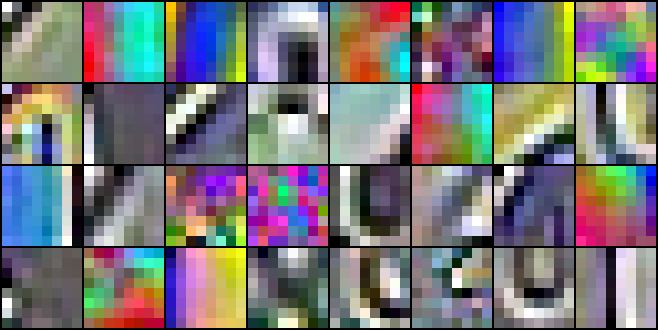
\includegraphics[width=\linewidth]{centroids.png}
  \caption{A selection of centroids generated when running the algorithm on the svhn~\cite{svhn} dataset.}
  \label{centroids}
\end{figure}

\subsection{Feature Extraction}

The algorithm then proceeds to extract features from images using the dictionary $\mathcal{D}$ as described in by the paper~\cite{paper} in section 4, and this is used to get the features to train a supervised model with and then classify future images. The algorithm takes one image at a time and extracts patches from that image of size $p\textrm{-by-}p$, starting from the top left and stepping along by some stride specified by the user. The pixel values are then extracted from the patches in same way as before and normalised using the same equation before being set as the columns of the matrix $P \in \mathbb{R}^{n \times w}$ where $w$ is the number of patches extracted from the image. These patches are then compared to the centroids by the calculation:
\[
F := \mathcal{D}^{\mathrm{T}}P
\]
where each column in the matrix represents a patch from the image and each value in the column is how closely that column matches the specific centroid.

\paragraph{}

The values from patches from $F$ are then pooled into groups of $u\textrm{-by-}u$, where $u$ is some user specified value, to reduce the number of features by $u^2$ fold. The pooling is done by simply summing the values in $F$ in the pool but with any negative values being treated as 0. All of these pooled values are then put into a final array of features which can then be used by some classification model.

\section{Experimental results}

Some results are shown in Table~\ref{table_ref}. These were generated using WEKA~\cite{weka}.

\begin{table}[h]
\footnotesize
\center
\begin{tabular}{|c|c|c|}
\hline
one column & another column & yet another column\\
one column & another column & yet another column\\
\hline
\end{tabular}
\caption{My table}
\label{table_ref}
\end{table}

\section{Conclusions}

Some conclusions here.

\bibliographystyle{plain}
\bibliography{report}

\end{document}
